\documentclass[10pt,a4paper]{article}
\usepackage{student}

% Metadata
\date{\today}
\setmodule{ELE2038: Signals and Control}
\setterm{Semester 2, 2025}

%-------------------------------%
% Other details
\title{Assignment H4}
\setmembername{David Thompson}
\setmemberuid{40401559}

%-------------------------------%
% Commands and packages
\usepackage{amsmath,amssymb,bm,physics,wrapfig}
\usepackage[backend=biber, style=ieee]{biblatex}
\addbibresource{ELE2038_H4.bib}
\nocite{*}

\graphicspath{ {plots/} }

\newcommand{\KL}{\mathrm{KL}}
\newcommand{\R}{\mathbb{R}}
\newcommand{\E}{\mathbb{E}}
\newcommand{\T}{\top}

\newcommand{\expdist}[2]{%
        \normalfont{\textsc{Exp}}(#1, #2)%
    }
\newcommand{\expparam}{\bm \lambda}
\newcommand{\Expparam}{\bm \Lambda}
\newcommand{\natparam}{\bm \eta}
\newcommand{\Natparam}{\bm H}
\newcommand{\sufstat}{\bm u}

%-------------------------------%
% Main document
\begin{document}
    \numberwithin{equation}{section}
    % Add header
    \header{}
    \section{Problem 1} 
        A system with a transfer function
        \begin{equation}
            G(s) = \frac{s^3 + s^2 - 5s -1}{8s^5 + 38s^4 + 65s^3 + 50s^2 + 17s + 2},
        \end{equation}
        can be shown to be BIBO-stable through the use of Routh's criterion. Defining $G$ as $G(s) = \frac{P(s)}{Q(s)}$, we can take $Q$ as the characteristic polynomial and construct a Routh's tabulation using its coefficients as shown in Table \ref{tb:rouths_Q}. When tabulated, it can be seen that all values in the first column are positive, therefore, all roots of $Q$ have a negative real part, meaning $G$ is BIBO-stable. $G$ can also be shown to be "sufficiently stable" if all of its poles are more than $0.2$ from the imaginary axis. We can show this by constructing another Routh's tabulation with the coefficients of $Q(s - c)$ where $c$ is the distance from the axis, in this case, $0.2$. If all values in the first column are positive, the poles of $G(s)$ are more than $0.2$ from the imaginary axis. Using the binomial theorem to expand $Q(s-c)$ and calculate the coefficients, 
        \begin{align}
            Q(s + 0.2) &= 8(s + 0.2)^5 + 38(s + 0.2)^4 + 65(s + 0.2)^3 + 50(s + 0.2)^2 + 17(s + 0.2) + 2 \\
            &= 8s^5 + 30s^4 + 37.8s^3 + 19.48s^2 + 3.648s + 0.138
        \end{align}
        Table \ref{tb:rouths_Qc} shows that this is the case, hence $G$ is BIBO-stable with all poles more than $0.2$ from the axis.
        \begin{table}[h]
            \centering
            \begin{tabular}{ c | c c c}
                $s^5$ & 8     & 65    & 17 \\
                $s^4$ & 38    & 50    & 2  \\
                $s^3$ & 54.47 & 16.58 & 0  \\
                $s^2$ & 38.43 & 2     & 0  \\
                $s^1$ & 13.74 & 0     & 0  \\
                $s^0$ & 2     & 0     & 0             
            \end{tabular}
            \caption{Routh's tabulation of $Q(s)$.}
            \label{tb:rouths_Q}
        \end{table}
        \begin{table}[h]
            \centering
            \begin{tabular}{ c | c c c}
                $s^5$ & 8     & 37.80 & 3.648 \\
                $s^4$ & 30    & 19.48 & 0.138 \\
                $s^3$ & 32.61 & 3.611 & 0     \\
                $s^2$ & 16.16 & 0.138 & 0     \\
                $s^1$ & 3.332 & 0     & 0     \\
                $s^0$ & 0.138 & 0     & 0             
            \end{tabular}
            \caption{Routh's tablulation of $Q(s + 0.2)$.}
            \label{tb:rouths_Qc}
        \end{table}

    \section{Problem 2}
        To tune a PID controller for the system
        \begin{equation} \label{eq:problem2}
            G(s) = \frac{0.5s + 1}{(s + 1)^3( 0.1s + 1)},
        \end{equation}
        various methods can be used.
    \subsection{Part (i)}
        First we will use the first Ziegler-Nichols method. We begin by finding the inflection point of the system's step response and plotting a tangent to the curve at that point. The plot of the step response and tangent are shown below in Figure \ref{fig:zn1_tangent}.
        \begin{figure}[h]
            \centering
            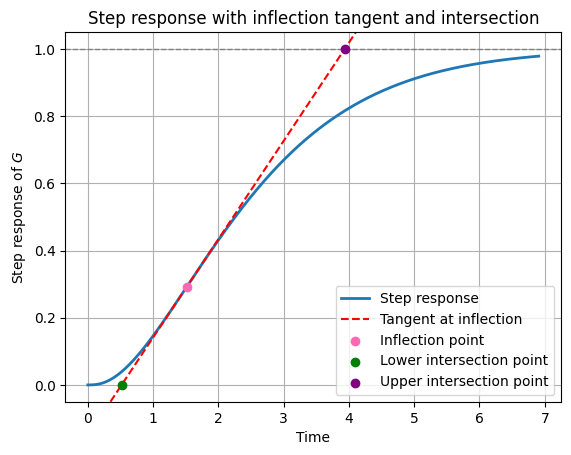
\includegraphics[width=0.5\textwidth]{zn1_stepRes+tangent.png}
            \caption{A plot of the step response of $G$ and a tangent to the curve at the inflection point.}
            \label{fig:zn1_tangent}
        \end{figure}
        We can then find the values required to calculate the tuning parameters given the two intersection points marked in Figure \ref{fig:zn1_tangent}. The resulting PID parameters are stated in Table \ref{tb:zn1_params} below.
        \begin{table}[h]
            \centering
            \begin{tabular}{ c | c | c }
                $K_c$ & $\tau_I$ & $\tau_D$ \\
                7.927 & 1.035    & 0.259
            \end{tabular}
            \caption{Ziegler-Nichols tuning parameters.}
            \label{tb:zn1_params}
        \end{table}
        Applying these parameters to the system in Equation (\ref{eq:problem2}) produces the step response shown in Figure \ref{fig:zn1_gcl}.
        \begin{figure}[h]
            \centering
            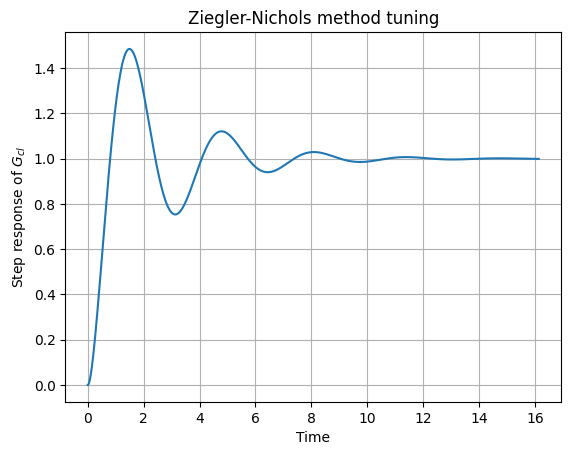
\includegraphics[width=0.5\textwidth]{zn1_Gcl.png}
            \caption{A plot of the step response of $G_{cl}$ tuned using the first Ziegler-Nichols method.}
            \label{fig:zn1_gcl}
        \end{figure}
    \subsection{Part (ii)}
        Second, we will use the Ziegler-Nichols ultimate sensitivity method. We start by finding the ultimate gain through experimentation, then we find the ultimate period. From these values we can calculate the PID controller parameters which are stated in Table \ref{tb:znu_params}.
        \begin{table}[h]
            \centering
            \begin{tabular}{ c | c | c }
                $K_p$ & $\tau_I$ & $\tau_D$ \\
                14.24 & 0.462    & 0.116
            \end{tabular}
            \caption{Ziegler-Nichols ultimate sensitivity method tuning parameters.}
            \label{tb:znu_params}
        \end{table}
        Applying these parameters to the system in Equation (\ref{eq:problem2}) produces the step response shown in Figure \ref{fig:znu_gcl}.
        \begin{figure}[h]
            \centering
            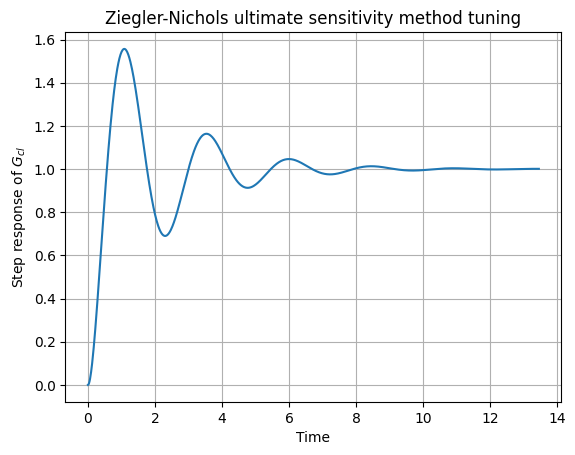
\includegraphics[width=0.5\textwidth]{znu_Gcl.png}
            \caption{A plot of the step response of $G_{cl}$ tuned using the Ziegler-Nichols ultimate sensitivity method.}
            \label{fig:znu_gcl}
        \end{figure}
        
    \section{Problem 3}
        The impulse response of a linear dynamical system is 
        \begin{equation}
            x(t) = 5 \sin(at + \frac{\pi}{4})e^{-2t} + 0.02H_{0.05}(t)e^{-0.2(t-0.5)},
        \end{equation}
        for $t >= 0$, for some constant $a$. We can test this impulse response to determine if the system is stable by verifying if the impulse response is absolutely integrable. Both terms of the expression contain an exponential decay factor which ensures that they are absolutely integrable over $[0, \infty)$. We can further show this by setting up the integration
        \begin{align}
            x(t) =& \int_{0}^{\infty} \left|5 \sin(at + \frac{\pi}{4})e^{-2t}\right|dt 
                + \int_{0}^{\infty} \left|0.02H_{0.05}(t)e^{-0.2(t-0.5)}\right|dt.
            \intertext{Considering the first term, since $\left|\sin(x) \le 1\right|$,}
            \implies & 5 \int_{0}^{\infty} e^{-2t}dt, \\
            =& 5 \left[-\frac{1}{2}e^{-2t}\right]_0^\infty, \\
            =& \frac{5}{2} < \infty.
            \intertext{Then, considering the second term, applying the Heaviside function}
            =& 0.02\int_{0.05}^{\infty} e^{-0.2(t-0.5)}dt,
            \intertext{substituting $u=t-0.5$}
            =& 0.02\int_{0}^{\infty} e^{-0.2u}du, \\
            =& 0.02\left[-\frac{1}{0.2}e^{-0.2u}\right]_0^\infty, \\
            =& 0.1 < \infty.
        \end{align}
        As both terms integrate to finite solutions, $x(t)$ is absolutely integrable and therefore the system is BIBO-stable.

    \section{{Problem 4}}
        A dynamical system with transfer function $G_s$, controlled by a PD controller with actuator and sensor transfer functions of $G_a = 1$ and $G_m = 1$ respectively, has a closed-loop transfer function, $G_{CL}$, of
        \begin{equation}
            G_{CL}(s) = \frac{K_C(1 + \tau_D s)G_s(s)}{1 + K_C (1 + \tau_D s) G_s(s)}.
        \end{equation}
        Where $K_C$ is the controller gain and $\tau_D$ is the time derivative constant. To find the offset of the system upon a step change of the set point, we can apply the final value theorem. We can do this as we can assume that $G_s$ is a proper rational function and is BIBO-stable, therefore all of its poles have a negative real part. Using a unit step input to model the change in set point; the output, $Y(s)$, would be
        \begin{equation}
            Y(s)=\frac{1}{s} \cdot G_{CL}(s).
        \end{equation}
        Therefore, applying the final value theorem and substituting $G_{CL}$
        \begin{align}
            \lim_{t \to \infty} y(t) =& \lim_{s \to 0} \frac{K_C (1 + \tau_D s) G_s(s)}{1 + K_C (1 + \tau_D s) G_s(s)},
            \intertext{applying the limit}
            \lim_{t \to \infty} y(t) =& \frac{K_C G_s(0)}{1 + K_C G_s(0)}. \label{eq:steadyState}
        \end{align}
        As $t$ approaches $\infty$, Equation (\ref{eq:steadyState}) equals the system's steady state value. As the offset is defined as the desired value, $1$, subtract the steady state value, Equation (\ref{eq:steadyState}), the offset is 
        \begin{equation} \label{eq:offset}
            \text{Offset} = 1 - \frac{K_C G_s(0)}{1 + K_C G_s(0)}.
        \end{equation}
    \printbibliography
\end{document}